\documentclass[10pt, landscape]{article}
\usepackage[scaled=0.92]{helvet}
\usepackage{calc}
\usepackage{multicol}
\usepackage[a4paper,margin=3mm,landscape]{geometry}
\usepackage{amsmath,amsthm,amsfonts,amssymb}
\usepackage{color,graphicx,overpic}
\usepackage{hyperref}
\usepackage{newtxtext} 
\usepackage{enumitem}
\usepackage[table]{xcolor}
\usepackage{mathtools}
\setlist{nosep}
% for including images
\graphicspath{ {./images/} }

\pdfinfo{
  /Title (MODULE_CODE.pdf)
  /Creator (TeX)
  /Producer (pdfTeX 1.40.0)
  /Author (Jovyn Tan)
  /Subject (MODULE_CODE)
/Keywords (MODULE_CODE, nus,cheatsheet,pdf)}

% Turn off header and footer
\pagestyle{empty}

% redefine section commands to use less space
\makeatletter
\renewcommand{\section}{\@startsection{section}{1}{0mm}%
  {-1ex plus -.5ex minus -.2ex}%
  {0.5ex plus .2ex}%x
{\normalfont\large\bfseries}}
\renewcommand{\subsection}{\@startsection{subsection}{2}{0mm}%
  {-1explus -.5ex minus -.2ex}%
  {0.5ex plus .2ex}%
{\normalfont\normalsize\bfseries}}
\renewcommand{\subsubsection}{\@startsection{subsubsection}{3}{0mm}%
  {-1ex plus -.5ex minus -.2ex}%
  {1ex plus .2ex}%
{\normalfont\small\bfseries}}%
\makeatother

\renewcommand{\familydefault}{\sfdefault}
\renewcommand\rmdefault{\sfdefault}
%  makes nested numbering (e.g. 1.1.1, 1.1.2, etc)
\renewcommand{\labelenumii}{\theenumii}
\renewcommand{\theenumii}{\theenumi.\arabic{enumii}.}
\renewcommand\labelitemii{•}
\renewcommand\labelitemiii{•}

\definecolor{mathblue}{cmyk}{1,.72,0,.38}
\everymath\expandafter{\the\everymath \color{mathblue}}

% Don't print section numbers
\setcounter{secnumdepth}{0}

\setlength{\parindent}{0pt}
\setlength{\parskip}{0pt plus 0.5ex}
%% adjust spacing for all itemize/enumerate
\setlength{\leftmargini}{0.5cm}
\setlength{\leftmarginii}{0.5cm}
\setlist[itemize,1]{leftmargin=2mm,labelindent=1mm,labelsep=1mm}
\setlist[itemize,2]{leftmargin=4mm,labelindent=1mm,labelsep=1mm}

% adding my commands
% tightcenter
\newenvironment{tightcenter}{%
  \setlength\topsep{0pt}
  \setlength\parskip{0pt}
  \begin{center}
    }{%
  \end{center}
}

% boxed
\newenvironment{tightbox}{%
  \setlength\topsep{0pt}
  \setlength\parskip{0pt}
  \begin{center}
    \begin{tabular}{|@{\hspace{\dimexpr\fboxsep+0.5\arrayrulewidth}}c@{\hspace{\dimexpr\fboxsep+0.5\arrayrulewidth}}|}
      \hline
    }
    {%
    \\ \hline
    \end{tabular}
  \end{center}
}

% fixed width box
\newenvironment{fixedbox}[1][0.7]{
  \setlength\topsep{0pt}
  \setlength\parskip{0pt}
  \begin{center}
    \begin{tabular}{|>{\centering\arraybackslash}m{#1\linewidth}|}
    \hline
  }{
  \\ \hline
  \end{tabular}
  \end{center}
}

% definition of a new term
\usepackage{soul}
\definecolor{paleyellow}{RGB}{251,243,218}
\newcommand{\definition}[2][]{\sethlcolor{paleyellow}\hl{\textbf{#2}} #1  $\rightarrow$}

% important note (attention)
\newcommand{\attention}{{\color{red}\textbf{! }}}



% -----------------------------------------------------------------------

\begin{document}
\raggedright
\footnotesize
\begin{multicols*}{4}
  % multicol parameters
  \setlength{\columnseprule}{0.25pt}

  \begin{center}
    \fbox{%
      \parbox{0.8\linewidth}{\centering \textcolor{black}{
          {\Large\textbf{CS3236}}
        \\ \normalsize{AY22/23 SEM 2}}
        \\ {\footnotesize \textcolor{gray}{github/jovyntls}}
      }%
    }
  \end{center}

  \section{00. INTRODUCTION}

  \subsection{data compression}

  \begin{itemize}
    \item types of compression
      \begin{itemize}
        \item \textbf{lossless compression} - can recover the contents
        \item \textbf{lossy compression} - lose some quality - cannot convert back to the higher-quality version
      \end{itemize}
    \item examples
      \begin{itemize}
        \item sparse binary string - storing positions of 1s
        \item equal number of 0/1s - $L \geq \log_2 \binom{64}{32} \approx 60.7$
        \item english text - using relative frequency
        \item morse code is NOT binary (contains spaces)
      \end{itemize}
    \item info theory uses \textbf{probabilistic models} (letter frequency, sequence probabilities)
    \item 2 distinct approaches to compression:
      \begin{itemize}
        \item \textbf{variable length} - map more probable sequences to shorter binary strings
        \item \textbf{fixed length} - map most probable sequences to strings of a given length
          \begin{itemize}
            \item insufficient strings for low-probability sequences 
            \item tradeoff between length/failure probability
          \end{itemize}
      \end{itemize}
  \end{itemize}

  \subsection{information theory concepts}
  \begin{itemize}
    \item speed: \definition{rate} $\frac{k}{n}$ (mapping $k$ bits to $n$ bits)
    \item reliability: $ \mathbb{P}[error] $ = $\mathbb{P}[\text{estimated msg $\neq$ true msg}]$
    \item \definition{source coding theorem} the fundamental compression limit is given by a source-dependent quantity known as the \textbf{(Shannon) entropy $H$}. The (average) storage length can be arbitrarily close to $H$, but can never be any lower than $H$.
      \begin{itemize}
        \item $H$ is a property of the \textit{probability distribution}
      \end{itemize}
    \item \definition{channel coding theorem} there exists a channel-dependent quantity called the \textbf{(Shannon) capacity $C$} such that arbitrarily small error probability can be achieved only for rates $<C$
      \begin{itemize}
        \item can achieve $ \mathbb{P}[error] \leq \epsilon \iff$ rate $<C$
      \end{itemize}
  \end{itemize}

  \subsection{data communication example}

  \begin{itemize}
    \item a "transmitter" sends a sequence of 0s and 1s
    \item a "receiver" sends a sequence \textit{with some corruptions}
  \end{itemize}

  \subsubsection{channel transition diagram}

  \begin{minipage}[c]{0.3\linewidth}
    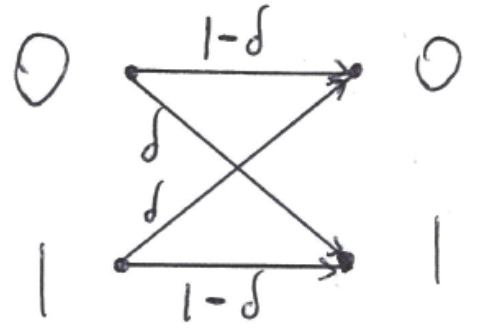
\includegraphics[width=0.8\linewidth]{cs3236-channel-transition-diagram.png} 
  \end{minipage}
  \begin{minipage}[c]{0.65\linewidth}
    \begin{itemize}
      \item each bit is flipped independently with probability $\delta \in (0, \frac{1}{2})$
    \end{itemize}
  \end{minipage}

  \subsubsection{naive}

  \begin{itemize}
    \item \textbf{uncoded communication} - $\mathbb{P}[correct] = (1-\delta)^N $
    \item \textbf{repetition code} - transmit "000" for "0", "111" for "1"
      \begin{itemize}
        \item $ \mathbb{P}[correct] = [(1-\delta)^3 + 3\delta(1-\delta)^2]^N $
        \item more reliable but 3x slower!
      \end{itemize}
  \end{itemize}

  \subsubsection{Hamming code}

  \begin{itemize}
    \item able to correct one bit flip
    \item maps binary string of length 4 to binary string of length 7
    \item fill in $b_1b_2b_3b_4$ and assign $c_1c_2c_3$ such that the sum of bits in each circle is even
      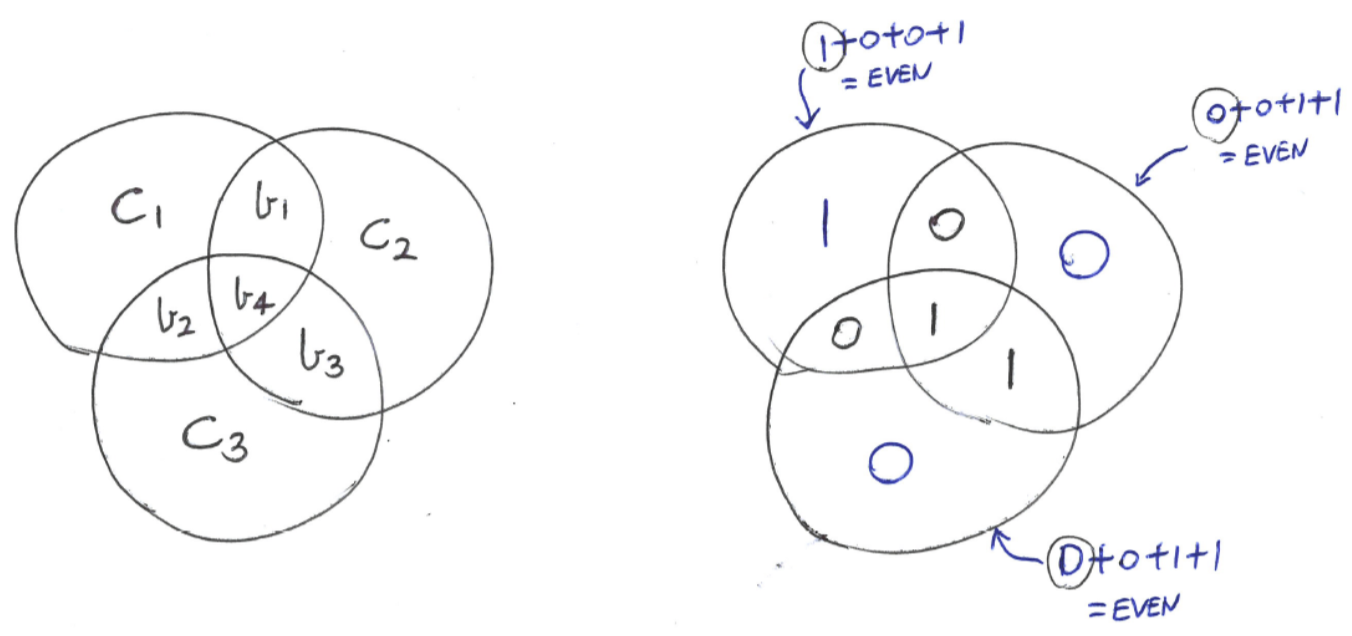
\includegraphics[width=0.8\linewidth]{cs3236-hamming-example.png} 
    \item $ \mathbb{P}[correct] \geq \mathbb{P}[\leq 1\text{bit flips}] = (1-\delta)^7 + 7\delta(1-\delta)^6 $
    \item with $\delta=1$: Shannon capacity $C\approx 0.531$ 
  \end{itemize}

  \section{01. INFORMATION MEASURES}

  \subsection{information of an event}

  \begin{itemize}
    \item \definition{entropy} measure of "uncertainty" or "information" in a random variable
    \item given event $A$ with some $\mathbb{P}[A] = p$, how much "information" learned by being told $A$ occurred?
      \begin{itemize}
        \item only $ \mathbb{P}[A] $ matters
      \end{itemize}
    \item if $A$ occurs with probability $p$, then $\quad Information(A) = \psi(p)$ for some function $\psi(\cdot)$
  \end{itemize}

  \subsubsection{axioms for $\psi(\cdot)$}

  \begin{tightcenter}
    \( {\displaystyle{ \psi(p) = \log_b \frac{1}{p} }} \) (for some base $b>0$)
  \end{tightcenter}

  we gain $\log_2 \frac{1}{p}$ "bits" of info if a probability-$p$ event occurs.

  \begin{minipage}[c]{0.3\linewidth}
    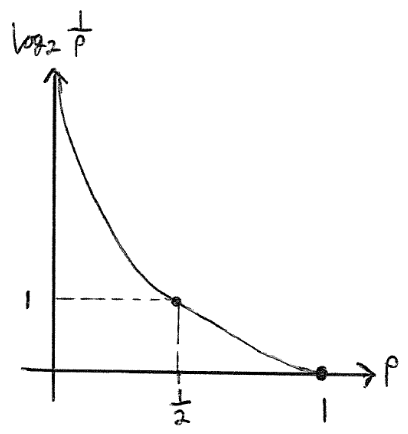
\includegraphics[width=0.95\linewidth]{cs3236-information-log2-p-graph.png} 
  \end{minipage}
  \begin{minipage}[c]{0.67\linewidth}
    \begin{itemize}
      \item only $\psi(p) = \log_b\frac{1}{p}$  satisfies all axioms
      \item we focus on $b=2$ 
        \begin{itemize}
          \item information measured in bits
        \end{itemize}
      \item all choices of $b$ are equivalent up to scaling by a universal constant
        \begin{itemize}
          \item e.g. \# of nats $= \log_e 2 \times$ \# of bits
        \end{itemize}
    \end{itemize}
  \end{minipage}

  \begin{enumerate}
    \item $\psi(p) \geq 0\quad$ (\textbf{non-negativity}) 
    \item $\psi(1) = 0\quad$ (\textbf{zero for definite events}) 
    \item if $p \leq p'$, then $\psi(p) \geq \psi(p') \quad$ (\textbf{monotonicity})
      \begin{itemize}
        \item the less likely an event is, the more information was learnt by the fact that it occurred
      \end{itemize}
    \item $\psi(p)$ in continuous in $p \quad$ (\textbf{continuity}) 
      \begin{itemize}
        \item small change in probability: no drastic change in info
      \end{itemize}
    \item $\psi(p_1 p_2) = \psi(p_1) + \psi(p_2)\quad$  
      \begin{itemize}
        \item (\textbf{additivity under independence}) if $A$ and $B$ are independent events with probabilities $p_1$ and $p_2$, then $\mathbb{P}[A \cap B]=p_1p_2$, and the information learnt from both $A$ and $B$ occurring is the sum of the two individual amounts of information (because they are independent)
        \item $\psi(\mathbb{P}[A_1 \cap A_2]) = \psi(\mathbb{P}[A_1]) + \psi(\mathbb{P}[A_2])$
      \end{itemize}
  \end{enumerate}


  \subsection{information of a random variable - entropy}

  \begin{itemize}
    \item let $X$ be a discrete r.v. with pmf $P_X$
    \item if we observe $X=x$ then we have learnt $\log_2 \frac{1}{P_X(x)}$ bits of information
  \end{itemize}

  \begin{tightcenter}
    \textbf{(Shannon) entropy} \\* is the average \textit{information/uncertainty} in $X$ wrt $P_X$:
    \begin{align*}
      H(X) &= \mathbb{E }_{X \sim P_X} \left[ \log_2 \frac{1}{P_X(X)} \right] 
        \\ &= \sum_x P_X(x) \log_2 \frac{1}{P_X(x)}
    \end{align*}
  \end{tightcenter}

  \begin{itemize}
    \item \definition{binary entropy function} \( {\displaystyle{ \quad\quad H_2(p) = p\log_2 \frac{1}{p} + (1-p) \log_2 \frac{1}{1-p} }} \) 
    \item e.g. 
      \begin{itemize}
        \item binary source: $X \sim Bernoulli(p)$, $\quad p \in (0,1)$ \\* $\quad \Rightarrow H(X) = H_2(p)$
        \item uniform source: $X$ is uniform on a finite set $\mathcal{X}$ 
          \begin{itemize}
            \item $P_X(x) = \frac{1}{\vert \mathcal{X} \vert}$
          \end{itemize}
          $\quad \Rightarrow$ $H(X) = \mathbb{E} \left[ \log_2 \frac{1}{1/\vert\mathcal{X}\vert} \right] = \log_2 \vert\mathcal{X}\vert$
      \end{itemize}
    \item entropy $\neq$ variance
      \begin{itemize}
        \item entropy depends \textit{only} on the probability values
      \end{itemize}
  \end{itemize}

  \subsubsection{axiomatic view (Shannon)}

  $X$ is a d.r.v. taking $N$ values with $\mathbf{p} = (p_1, \dots, p_N)$. We consider a general information measure of the form 
  \centerline{$\Phi(\mathbf{p}) = \Phi (p_1, \dots, p_N)$}

  \begin{tightcenter}
    only  $\Phi(X) = constant \times H(X)$ satisfies all axioms.
  \end{tightcenter}

  \begin{enumerate}
    \item $\Psi(\mathbf{p})$ is continuous on $p \quad$ (\textbf{continuity}) 
    \item if $p_i= \frac{1}{N}$, then $\Psi(\mathbf{p}) $ is increasing in $N$ (\textbf{uniform case})
      \begin{itemize}
        \item uniformity over a larger set of outcomes always means more uncertainty
      \end{itemize}
    \item (\textbf{successive decisions}) $\Psi(p_1, \dots, p_N) = \Psi(p_1 + p_2, p_3, \dots, p_N) + (p_1 + p_2) \Psi (\frac{p_1}{p_1 + p_2}, \frac{p_2}{p_1 + p_2})$
  \end{enumerate}

  \subsubsection{variations}

  \begin{itemize}
    \item \definition[ of two random variables $(X, Y)$ ]{joint entropy}
      \begin{align*}
        H(X,Y) &= \mathbb{E}_{(X, Y)\sim P_{XY}} \left[ \log_2 \frac{1}{P_{XY}(X,Y)} \right] 
            \\ &= \sum_{x,y} P_{XY} (x,y) \log_2 \frac{1}{P_{XY}(x,y)}
      \end{align*}
    \item \definition[ of $Y$ given $X$ ]{conditional entropy}
      \begin{align*}
        H(Y\vert X) &= \mathbb{E}_{(X,Y) \sim P_{XY}} \left[ \log_2 \frac{1}{P_{Y\vert X}(Y\vert X)} \right] 
                 \\ &= \sum_{x, y} P_{XY}(x,y) \log_2  \frac{1}{P_{Y\vert X}(y\vert x)}
                 \\ &= \sum_x P_X(x) H(Y \vert X=x)
      \end{align*}
      \begin{itemize}
        \item on average, knowing $X$ reduces uncertainty about $Y$ ($H(Y\vert X) \leq H(Y)$), but seeing a \textit{specific} outcome of $X$ may increase uncertainty about $Y$ ($H(Y \vert X=i) > H(Y)$ for some values of $i$)
      \end{itemize}
  \end{itemize}

  \subsection{properties of entropy}

  \begin{enumerate}
    \item $H(X) \geq 0 \quad$ (\textbf{non-negativity})
      \begin{itemize}
        \item $H(X)=0 \iff X$ if deterministic
        \item proof: information $\log_2\frac{1}{p} \geq 0$ for $p \in [0,1]$, so entropy is the average of a non-negative quantity, and itself is non-negative
      \end{itemize}
    \item $H(X) \leq \log_2 \vert\mathcal{X}\vert \quad$ (\textbf{upper bound}) \\* if $X$ takes values on a finite alphabet $ \mathcal{X} $
      \begin{itemize}
        \item $H(X) = \log_2\vert \mathcal{X}\vert \iff X\sim Uniform(\mathcal{X})$
        \item implies $\quad H(X \vert Y) \leq \log_2 \vert \mathcal{X} \vert$
      \end{itemize}
    \item $H(X, Y) = H(X) + H(Y\vert X) \quad$ (\textbf{chain rule})
      \begin{itemize}
        \item or $H(X, Y) = H(Y) + H(X\vert Y)$
        \item overall information in $(X, Y)$ is the information in $X$ plus the remaining information in $Y$ after observing $X$.
        \item general chain rule: $H(X_1, \dots, X_n) = \sum^n_{i=1} H(X_i \vert X_1, \dots, X_{i-1})$
      \end{itemize}
    \item $H(X \vert Y) \leq H(X) \quad$ (\textbf{conditioning reduces entropy})
      \begin{itemize}
        \item $H(X \vert Y) = H(X) \iff X$ and $Y$ are independent
        \item additional information $Y$ can't increase uncertainty \textit{on average}
        but \textit{can} have $H(X \vert Y=y) > H(X)$
      \end{itemize}
    \item $H(X_1, \dots, X_n) \leq \sum^n_{i=1} H(X_i) \quad$ (\textbf{sub-additivity})
      \begin{itemize}
        \item equality $\iff X$ and $Y$ are independent
      \end{itemize}
  \end{enumerate}


\end{multicols*}

\end{document}
